\documentclass[a4paper, oneside]{article} 
\usepackage{tikz}
\usepackage{amsmath}
\usepackage{amssymb}
\usepackage{graphicx}
\usepackage{hyperref}
\usepackage{enumitem}
\usepackage{nicefrac}
\usepackage{empheq}
\usepackage{xcolor}
\usepackage{array}
\usepackage{indentfirst}
\usepackage{enumitem}
\usepackage[fancysections,  titlepage, pagenumber]{polytechnique}
\usepackage{float}

\title[C.A.S.T.L.E]{Market Design Project: C.A.S.T.L.E}
\subtitle{Capacity-Alligned Stable Teaching Location Engine\\
Tackling classroom allocation in Universities}
\author{Matthieu MINGUET}
\date{December 2024}

\begin{document}
\maketitle

\section{Executive Summary}
\pagebreak

\tableofcontents
\pagebreak

\section{Introduction}
The way the rooms are organized leads to inefficiencies, between professors who value and need different things. Some professors need to use boards to write specific, while others do not value such things. Moreover, the impact of the geographical positioning of the rooms relative to both the students and the teachers is something to take into consideration, or the proximity of the coffee machine, even the amount of stairs required to reach the room.
As such it is my belief that a new system designed around the principles of market design could lead to a more efficient allocation of the school’s resources, as well as collect valuable information term on term on what professors value and what type of classrooms they preconize.
\pagebreak

\section{Due Diligence}
\subsection{Current System at Ecole Polytechnique}
X currently operates a centralized room allocation system managed by the Registrar's office through a shared spreadsheet.
While the basic objective of assigning rooms to all classes is met, the system faces significant operational challenges.
The manual allocation process is time-consuming, requires frequent bargaining between departments, and often fails to meet teacher preferences and specific classroom needs.
Moreover, it does not provide a reporting of what the

The system's current stability relies heavily on the natural distribution of class sizes, particularly in the \textit{Cycle Ingénieur} program where enrollment decreases
from 550 students in first year to increasingly smaller specialized groups through second and third year. This pattern allows for predictable allocations, such as Poincare for large
lectures and smaller rooms for tutorials, especially when third-year students are off-campus. With the inversion of tutorials and lectures times based on the year, the system can support
the needs of the program.

However, mounting pressure from expanding masters and bachelor programs is straining this delicate balance. The competition for rooms,
especially between second and third-year needs, is intensifying. While the system functions now due to fortunate enrollment patterns,
it lacks the robustness to handle future growth and increasing complexity.

\subsubsection{Flaws in the current system}
In terms of market design, this system is a centralized dictatorship, as in a control economy where resources are allocated based on the sole criteria of class size. It's flaws which we will detail in the following table:\\

\begin{tabular}{|p{2.5cm}|p{10cm}|>{\centering\arraybackslash}p{2.5cm}|}
	\hline
	\textbf{Flaw}                                                                                 & \textbf{Description} & \textbf{Intensity} \\
	\hline
	Information Problem                                                                           &
	\begin{itemize}[leftmargin=*,nosep,topsep=0pt,partopsep=0pt,before=\vspace{-\baselineskip}]
		\item No preference elicitation
		\item Manual spreadsheet means no way to communicate preferences, constraints, or trade
	\end{itemize}     &
	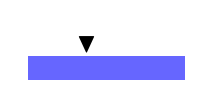
\begin{tikzpicture}
		\fill[blue!60] (0,0) rectangle (2,0.3);
		\node[anchor=center] at (0.75,0.45) {$\blacktriangledown$};
	\end{tikzpicture}                                                                                \\[2ex]
	\hline
	Matching Mechanism                                                                            &
	\begin{itemize}[leftmargin=*,nosep,topsep=0pt,partopsep=0pt,before=\vspace{-\baselineskip}]
		\item Single-Criterion Optimization: capacity matching
		\item Manual Coordination Cost: bargaining
		\item No formal Trading Mechanism: no beneficial trades
	\end{itemize}     &
	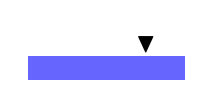
\begin{tikzpicture}
		\fill[blue!60] (0,0) rectangle (2,0.3);
		\node[anchor=center] at (1.5,0.45) {$\blacktriangledown$};
	\end{tikzpicture}                                                                                 \\[2ex]
	\hline
	Incentive Problems                                                                            &
	\begin{itemize}[leftmargin=*,nosep,topsep=0pt,partopsep=0pt,before=\vspace{-\baselineskip}]
		\item No strategic reporting: no formal way to express the preferences for rooms or features
		\item Lack of Price Mechanism: no way of quantifying preferences
	\end{itemize}  &
	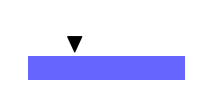
\begin{tikzpicture}
		\fill[blue!60] (0,0) rectangle (2,0.3);
		\node[anchor=center] at (0.6,0.45) {$\blacktriangledown$};
	\end{tikzpicture}                                                                                 \\[2ex]
	\hline
	Scalability                                                                                   &
	\begin{itemize}[leftmargin=*,nosep,topsep=0pt,partopsep=0pt,before=\vspace{-\baselineskip}]
		\item Brittle equilibrium: program change or growth could pose a threat to the current system
		\item Manual processing bottleneck
	\end{itemize} &
	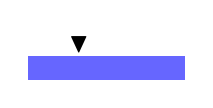
\begin{tikzpicture}
		\fill[blue!60] (0,0) rectangle (2,0.3);
		\node[anchor=center] at (0.65,0.45) {$\blacktriangledown$};
	\end{tikzpicture}                                                                                \\[2ex]
	\hline
	Efficiency problem                                                                            &
	\begin{itemize}[leftmargin=*,nosep,topsep=0pt,partopsep=0pt,before=\vspace{-\baselineskip}]
		\item No Optimization Algorithm
		\item Suboptimal Outcomes: room for Pareto improvements
		\item Resource Utilization: inefficient use of features and capabilities
	\end{itemize}    &
	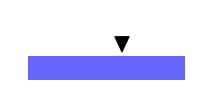
\begin{tikzpicture}
		\fill[blue!60] (0,0) rectangle (2,0.3);
		\node[anchor=center] at (1.2,0.45) {$\blacktriangledown$};
	\end{tikzpicture}                                                                                 \\[2ex]
	\hline
	Adaptation and flexibility                                                                    &
	\begin{itemize}[leftmargin=*,nosep,topsep=0pt,partopsep=0pt,before=\vspace{-\baselineskip}]
		\item Rigid system: changes mid-term can be difficult
		\item Limited feedback loop: for allocation and features
	\end{itemize}    &
	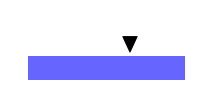
\begin{tikzpicture}
		\fill[blue!60] (0,0) rectangle (2,0.3);
		\node[anchor=center] at (1.3,0.45) {$\blacktriangledown$};
	\end{tikzpicture}                                                                                 \\[2ex]
	\hline
\end{tabular}
\linebreak

\vspace{0.05cm}

As we can see, while the current system has major flaws like the lack of a matching mechanism,
it still ensures all teachers have a room, and the school has functioned with this system for the past few years without any issues,
especially when the \textit{Cycle Ingénieur} program was the only program at the school.

\subsection{Current system at Clermont School of Business (Clermont SB)}
The Clermont SB has a similar system to Ecole Polytechnique, with a centralized room allocation and planning system. A dedicated member of staff is responsible
for managing the system in place: Program Directors submit room requirement and planning forms to the Planning Office, which then manually attributes the rooms based on the information provided,
and the availabilities of the rooms.

While the system allows for inputs from the faculty, the major issue si that the large number of programs and the increasing number of students in each program
is making the system increasingly complex to manage by hand and is leading to inefficiencies and tensions in the allocation. Moreover, this system is quite slow and requires
a large amount of time to manage, which could be streamlined and better used elsewhere. Finally, the system is not transparent,
and the faculty does not have a clear understanding of how the rooms are allocated, while it also doesn't encourage truthful reporting of preferences.

\subsubsection{Flaws in the current system}
Similarly as what we did for Ecole Polytechnique, we have identified the following flaws in the current system at Clermont SB:\\

\begin{tabular}{|p{2.5cm}|p{10cm}|>{\centering\arraybackslash}p{2.5cm}|}
	\hline
	\textbf{Flaw}                                                                              & \textbf{Description} & \textbf{Intensity} \\
	\hline
	Information Problem                                                                        &
	\begin{itemize}[leftmargin=*,nosep,topsep=0pt,partopsep=0pt,before=\vspace{-\baselineskip}]
		\item Preference reporting through requirement forms
		\item Lack of transparency in allocation process
	\end{itemize} &
	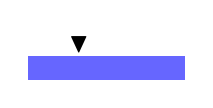
\begin{tikzpicture}
		\fill[blue!60] (0,0) rectangle (2,0.3);
		\node[anchor=center] at (0.65,0.45) {$\blacktriangledown$};
	\end{tikzpicture}                                                                             \\[2ex]
	\hline
	Matching Mechanism                                                                         &
	\begin{itemize}[leftmargin=*,nosep,topsep=0pt,partopsep=0pt,before=\vspace{-\baselineskip}]
		\item Manual attribution based on submitted forms
		\item Single-person decision making process
		\item No formal mechanism for resolving conflicts
	\end{itemize} &
	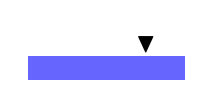
\begin{tikzpicture}
		\fill[blue!60] (0,0) rectangle (2,0.3);
		\node[anchor=center] at (1.5,0.45) {$\blacktriangledown$};
	\end{tikzpicture}                                                                              \\[2ex]
	\hline
	Incentive Problems                                                                         &
	\begin{itemize}[leftmargin=*,nosep,topsep=0pt,partopsep=0pt,before=\vspace{-\baselineskip}]
		\item No incentive for truthful preference reporting
		\item Lack of feedback mechanism
	\end{itemize} &
	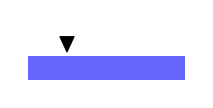
\begin{tikzpicture}
		\fill[blue!60] (0,0) rectangle (2,0.3);
		\node[anchor=center] at (0.5,0.45) {$\blacktriangledown$};
	\end{tikzpicture}                                                                              \\[2ex]
	\hline
	Scalability                                                                                &
	\begin{itemize}[leftmargin=*,nosep,topsep=0pt,partopsep=0pt,before=\vspace{-\baselineskip}]
		\item Growing complexity with increasing programs
		\item Rising student numbers strain current system
		\item Single point of failure (dedicated staff member)
	\end{itemize} &
	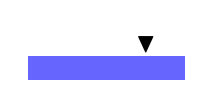
\begin{tikzpicture}
		\fill[blue!60] (0,0) rectangle (2,0.3);
		\node[anchor=center] at (1.5,0.45) {$\blacktriangledown$};
	\end{tikzpicture}                                                                              \\[2ex]
	\hline
	Efficiency problem                                                                         &
	\begin{itemize}[leftmargin=*,nosep,topsep=0pt,partopsep=0pt,before=\vspace{-\baselineskip}]
		\item Time-intensive manual process
		\item Inefficiencies in allocation
		\item Resource under-utilization due to information gaps
	\end{itemize} &
	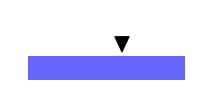
\begin{tikzpicture}
		\fill[blue!60] (0,0) rectangle (2,0.3);
		\node[anchor=center] at (1.2,0.45) {$\blacktriangledown$};
	\end{tikzpicture}                                                                             \\[2ex]
	\hline
	Adaptation and flexibility                                                                 &
	\begin{itemize}[leftmargin=*,nosep,topsep=0pt,partopsep=0pt,before=\vspace{-\baselineskip}]
		\item System struggles with program diversity
		\item Difficult to make mid-term adjustments
		\item Slow response to changing needs
	\end{itemize} &
	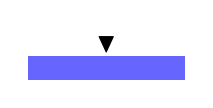
\begin{tikzpicture}
		\fill[blue!60] (0,0) rectangle (2,0.3);
		\node[anchor=center] at (1,0.45) {$\blacktriangledown$};
	\end{tikzpicture}                                                                             \\[2ex]
	\hline
\end{tabular}
\end{document}